\section{The idea}
\label{sec:theidea}

The idea appeared as part of the daily life of a normal student. Students in general, do not have a large budget for buying luxury ingredients to make interesting meals. However, eating pasta and ketchup seven days a week is not fun. So the motivation for this project was how to plan something interesting for dinner while staying on a low budget. 

The problem can be solved by using two existing software solutions, but we found no application that combines the two, to make a complete service.

Below is listed two motivational scenarios for making this application, and show . The first is: you just got off the university and you walk into a grocery store to pick up items to make dinner. You are tired and have trouble working out what to make. This is when you pull out your mobile phone and open \todo{BilligAftensmad?}. The application knows your taste and uses GPS-location to figure out which grocery store you are in. It will now provide you with a list of recipes matching your taste and searching criteria, from which you can gain inspiration or fully commit to cooking a certain recipe. The application will give you a list of ingredients to buy, and how to prepare and cook the meal.

The second scenario is: you are sitting a home planing your dinners for the following week. You are trying to make ends meet on a low budget, therefore you want to buy cheap meals but additionally want some healthy and quality food. You use \todo{BilligAftensmad?} to search for cheap recipes in a five kilometer radius around your place and you look where you can pick the ingredients for these recipes up, saving the most possible money. It is optional, but if you want the application to help you picking healthy food, you search for the recipe tag \textit{healthy}, and you will be provided with healthy recipes.

\begin{figure}[H]
	\centering
	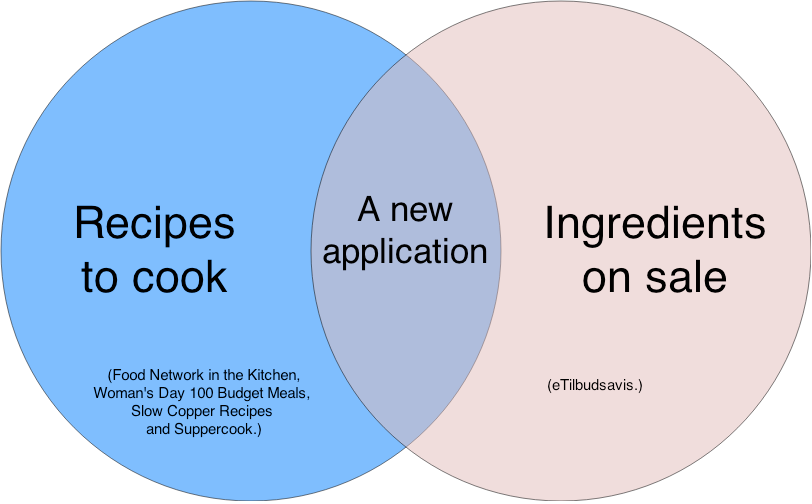
\includegraphics[width=0.7\textwidth]{Pictures/theideadiagram.png}
	\caption{Diagram showing the coupling of two fields, to make a new innovative application.}
	\label{fig:theideaasdiagram}
\end{figure}

The motivation for this application is providing existing services in a combined form and attach more opportunities regarding search, sorting and preferences to this combined application. Figure \ref{fig:theideaasdiagram} shows how the two existing services are coupled to form a new application.